        %%******************************************%%
        %%                                          %%
        %%        Modello di tesi di laurea         %%
        %%            di Andrea Giraldin            %%
        %%                                          %%
        %%             2 novembre 2012              %%
        %%                                          %%
        %%******************************************%%

\begin{document}
    \frontmatter
    \begin{titlepage}
    \begin{center}
        \begin{LARGE}
            \textbf{\myUni}\\
        \end{LARGE}

        \vspace{10pt}

        \begin{Large}
            \textsc{\myDepartment}\\
        \end{Large}

        \vspace{10pt}

        \begin{large}
            \textsc{\myFaculty}\\
        \end{large}

        \vspace{30pt}
        \begin{figure}[htbp]
            \centering
            
\includegraphics[height=6cm]{unipd-logo}
        \end{figure}
        \vspace{30pt}

        \begin{LARGE}
            \textbf{\myTitle}\\
        \end{LARGE}

        \vspace{10pt}

        \begin{large}
            \textsl{\myDegree}\\
        \end{large}

        \vspace{40pt}

        \begin{large}
            \begin{flushleft}
                \textit{Relatrice}\\
                \vspace{5pt}
                \profTitle\ \myProf
            \end{flushleft}

            % You can tweak the spacing to have professor and student names on the same line
            % useful if the page is broken by a long thesis title and you need more space
            % \vspace{-52pt}

            \begin{flushright}
                \textit{Laureando}\\
                \vspace{5pt}
                \myName \\
                \vspace{5pt}
                Matricola: \myMatricola
            \end{flushright}
        \end{large}

        \vspace{28pt}

        \line(1, 0){338} \\
        \begin{normalsize}
            \textsc{Anno Accademico \myAA}
        \end{normalsize}
    \end{center}
\end{titlepage}

    \clearpage
\phantomsection
\thispagestyle{empty}

\hfill
\vfill

\noindent\myName: \textit{\myTitle,}
\myDegree,
\textcopyright\ \myTime.

    \cleardoublepage
\phantomsection
\thispagestyle{empty}
\pdfbookmark{Dedica}{Dedica}

\vspace*{3cm}

\begin{center}
    Leave a Little Sparkle wherever you go. \\ \medskip
\end{center}

\medskip

\begin{center}
    Dedicato a tutti coloro che ci sono stati vicini nei momenti più difficili.
\end{center}

    \cleardoublepage
\phantomsection
\pdfbookmark{Sommario}{Sommario}
\begingroup
\let\clearpage\relax
\let\cleardoublepage\relax
\let\cleardoublepage\relax

\chapter*{Sommario}

Il presente documento descrive il lavoro svolto durante il periodo di stage, della durata di circa trecento ore, dal laureando Marco Brugin presso l'azienda Sybclab S.r.L.
Gli obbiettivi da raggiungere sono stati:
in primo luogo è stata richiesta la comprensione dei vantaggi e degli overhead portati da una architettura Event Driven,
in secondo luogo è stata richiesta la comprensione e implementazione di una data pipeline con il trattamento dei dati tramite Apache Kafka e Apache Druid ed infine la comprensione e la gestione gestione delle Time Series e dei Column-based Databases.
Il prototipo sviluppato presenterà una architettura distribuita, ad alta affidabilità, scalabile e resiliente, eseguibile tramite Docker Compose.
%\vfill

%\selectlanguage{english}
%\pdfbookmark{Abstract}{Abstract}
%\chapter*{Abstract}

%\selectlanguage{italian}

\endgroup

\vfill

    \cleardoublepage
\phantomsection
\pdfbookmark{Ringraziamenti}{ringraziamenti}

\begin{flushright}{
    \slshape
    ``Life is really simple, but we insist on making it complicated''} \\
    \medskip
    --- Confucius
\end{flushright}


\bigskip

\begingroup
\let\clearpage\relax
\let\cleardoublepage\relax
\let\cleardoublepage\relax

\chapter*{Ringraziamenti}

\noindent \textit{Innanzitutto, vorrei esprimere la mia gratitudine al Prof. \myProf, relatore della mia tesi, per l'aiuto e il sostegno fornitomi durante la stesura del lavoro.}\\

\noindent \textit{Desidero ringraziare con affetto i miei genitori per il sostegno, il grande aiuto e per essermi stati vicini in ogni momento durante gli anni di studio.}\\

\noindent \textit{Ho desiderio di ringraziare poi i miei amici per tutti i bellissimi anni passati insieme e le mille avventure vissute.}\\
\bigskip

\noindent\textit{\myLocation, \myTime}
\hfill \myName

\endgroup

    \cleardoublepage
\pdfbookmark{\contentsname}{tableofcontents}
\setcounter{tocdepth}{2}
\tableofcontents
%\markboth{\contentsname}{\contentsname}
\clearpage

\begingroup
    \let\clearpage\relax
    \let\cleardoublepage\relax
    \let\cleardoublepage\relax

    % Figures list
    \phantomsection
    \pdfbookmark{\listfigurename}{lof}
    \listoffigures

    \vspace*{8ex}

    % Tables list
    \phantomsection
    \pdfbookmark{\listtablename}{lot}
    \listoftables

    \vspace*{8ex}
\endgroup

\cleardoublepage

    \cleardoublepage

    \mainmatter
    \chapter{Introduzione}
\label{cap:introduzione}
\section{Descrizione dell'azienda}
Sync Lab s.r.L. è una azienda italiana attiva nell'abito \gls{ict}{}, specializzata nello sviluppo e consulenza IT dal 2002 con sedi a 
Milano, Roma, Napoli, Verona e Como. È una azienda orientata verso la Business Innovation, finalizzata alla 
creazione di soluzioni innovative che abbracciano i nuovi paradigmi della trasformazione digitale.
Sync Lab possiede numerose certificazioni ISO LL-C per l'attestazione della 
qualità dei prodotti e servizi offerti. In particolare possiede le certificazioni 
ISO-9001 per la qualità dell'azienda, ISO-14001 per l'adozione quadro sistematico per l'integrazione delle pratiche a protezione dell'ambiente, ISO-27001 per la definizione di un \gls{sgsi}{}, ISO-45001 per l'adozione di un \gls{ohs}{}.
\\
Attualmente Sync Lab dal punto di vista dell'organico è composta da più 300 dipendenti e lavora per più di 150 clienti diretti e finali, tra i più rilevanti ci sono nomi come: TIM, Trenitalia, PosteItaliane, UniCredit, ENI, ENEL, Vodafone, Fastweb.
\\
Sync Lab è un'azienda che si pone come obiettivo quello di essere un punto di riferimento per i propri clienti nella realizzazione di prodotti e soluzioni innovative per diversi settori di mercato, come mostrato  tra i quali: Sanità, Industria, Energia, Telco, Finanza e Trasporti \& Logistica.\\
Lo spirito di Sync Lab è ampiamente rappresentato dal logo aziendale Figura \ref{figure:logo_azienda}, che rappresenta un'onda che si propaga in modo circolare, che simboleggia la capacità di adattarsi e di evolversi in modo continuo.\\


\begin{figure}[htbp]  
\centering
    
\includegraphics[width=0.5\textwidth]{images/introduzione/logo_azienda.png}
    \caption{Logo dell'aziedan Sync Lab s.r.L.}
    \label{figure:logo_azienda}
\end{figure}
\pagebreak
\section{Idea di fondo del progetto}
Oggigiorno la gestione e l'analisi di grandi moli di dati in tempo reale sta diventando fondamentale 
per le aziende che vogliono rimanere competitive sul mercato. \\ 
Per questo motivo è necessario utilizzare tecnologie e software che permettano di analizzare e archiviare 
i dati in modo efficiente e veloce. \\
D'altro canto, però, è necessario anche che queste tecnologie siano in grado di scalare in modo verticale e orizzontale in base al carico 
di lavoro da sostenere. Inoltre è necessario che queste tecnologie siano in grado di garantire un elevato livello affidabilità. \\
Per questo motivo Sync Lab ha deciso d' investire in un progetto di ricerca e sviluppo che ha come obiettivo quello di creare 
una \gls{Data Pipeline}{} in grado di garantire le caratteristiche sopra descritte. \\
L'azienda ha già a disposizione un sistema di raccolta dati in  real time, basato su Apache Kafka, che permette di ricevere dati da
diversi sistemi e applicazioni, ma vuole andarlo a integrare con un sistema di analisi in real time permetta di eseguire operazioni 
sui dati ricevuti prima di archiviarli. \\
Particolarmente importante dovrà essere la fase di analisi dei dati, in quanto dovrà essere possibile eseguire operazioni di aggregazione
per aumentare la successiva estrazione dei dati. 
\subsection{Il ruolo dello stagista}
Lo stagista ha un ruolo fondamentale in tale tipologia di progetto, infatti è colui che porta uno spirito d'innovazione e consolida il valore aggiunto 
aziendale. \\
Le attività che costituiscono il percorso che lo stagista ha intrapreso sono state elencate all'interno di un \textit{Piano di lavoro}, che ha aiutato il tutor 
aziendale designato da Sync Lab a guidare e valutare il lavoro svolto dallo stagista. \\
Inoltre al termine del periodo di stage, sotto la supervisione del tutor aziendale è stata pianificata una presentazione rivolta a tutti \textit{stakeholder} aziendali, mirata a 
mostrare i risultati ottenuti con le tecnologie utilizzate e mettere in risalto le potenzialità del prototipo sviluppato. D'altra parte tale presentazione è stata anche l'occasione 
per un confronto per far emergere eventuali criticità o difetti,  e miglioramenti da apportare al prototipo sviluppato.
\pagebreak
\section{Il progetto di stage}
\subsection{Descrizione del progetto}
Le attività descritte in questa tesi si basano sulla progettazione e realizzazione di un prototipo di \gls{Data Pipeline}{} in grado di ricevere dati in real time da un sistema di raccolta dati basato su Apache Kafka, eseguire operazioni di aggregazione con Apache Druid in modo efficiente per facilitarne la successiva estrazione, fornendo così in output dati pronti per l'analisi.\\
In generale una \gls{Data Pipeline}{} è costituita da tre elementi sostanziali: una origine, una o più fasi di trasformazione e una o più destinazioni.
Inoltre per facilitare le operazioni di deploy è richiesto che il prototipo sia eseguibile con Docker Compose. \\
Il progetto in sè fa parte di una rivoluzione tecnologica che Sync Lab sta portando avanti nel campo \gls{Data Processing}{} e \gls{Data Analytics}{}. \\
In particolare il progetto di stage si pone come obiettivo quello di andare ad analizzare le prestazioni di Apache Druid rispetto ad un classico database relazionale, come PostgreSQL, in termini di velocità di esecuzione delle query e di scalabilità in relazione alle funzionalità di aggregazione fornite da tale strumento. 
\subsection{Obiettivi formativi}
In generale lo stage ha come obiettivo quello di far acquisire allo stagista concetti fondamentali riguardanti: 
\begin{itemize}
    \item Container technology;
    \item Apache Kafka e le Event Driven Architecture, design publish/subscribe;
    \item Column Based Database e la relazione/confronto tra questi e i classici DB relazionali SQL e quelli
    Documentali;
    \item Middleware, \gls{Data Pipeline}{}, le architetture distribuite, scalabili e resilienti.
\end{itemize}
\subsection{Risultati attesi e Obiettivi fissati}
Sono riportati nella Tabella \ref{tab:Tabella1} i risultati attesi e gli obiettivi fissati per lo stage con rispettivo identificativo, importanza e breve descrizione.
L'identificativo (riportato in breve con “ID”) è la sigla che identifica ogni requisito e rispetta la seguente notazione [Importanza][Identificativo]. \\
L’importanza è indicata dalla sigla O oppure F ad indicare rispettivamente un obiettivo
obbligatorio oppure facoltativo; mentre l’identificativo è un numero incrementale che
segnala in modo univoco l’obiettivo o il risultato in esame.\\
\\
Ogni obiettivo è identificato, o risultato viene classificato secondo l'importanza in: 
\begin{list}{*}{}
    \item \textbf{Obbligatorio (O)}: obiettivo irrinunciabile, vincolante in quanto necessario per l'avanzamento del progetto;
    \item \textbf{Facoltativo (F)}: obiettivo utile ma non essenziale, che può essere soddisfatto solo se tutti gli obiettivi obbligatori sono stati raggiunti e il cui soddisfatto rende il progetto più completo.     
\end{list} 

 \begin{table}[htbp]
    \centering
    \caption{Tabella degli obiettivi}    
    \label{tab:Tabella1}
    \begin{tabularx}{\textwidth}{|c|c|X|}
        \hline
        \textbf{ID} & \textbf{Importanza} & \textbf{Descrizione} \\\hline
        O1 & Obbligatorio & comprensione e definizione di una piccola \gls{Data Pipeline}{}  che  preveda il trattamento dei dati
        tramite Apache Kafka e Apache Druid \\\hline
        O2 & Obbligatorio & comprensione dei vantaggi e degli overhead  che le Event Driven Architecture portano con
        sé\\\hline
        O3 & Obbligatorio & comprensione del pattern publisher/subscriber \\\hline
        O4 & Obbligatorio & set-up di un cluster Apache Kafka in ambiente  containerizzato \\\hline
        O5 & Obbligatorio & gestione delle Time Series e dei Column-based Databases \\\hline
        O6 & Obbligatorio & comprensione delle differenze tra i database relazionali  classici e i Column-based Databases\\\hline
        O7 & Obbligatorio &comprensione dell’impiego e utilità dei middleware \\\hline
        F1 & Facoltativo & produzione di documentazione e un pacchetto di configurazione  dell’ambiente di sviluppo e
        esecuzione  della \gls{Data Pipeline}{}\\\hline
        F2 & Facoltativo & produzione di documentazione che riporti  le differenze  di performance  tra Apache Druid e altri
         database relazionali classici per alcune  operazioni \gls{olap}{} \\\hline
        F3 & Facoltativo & realizzazione di una presentazione che illustri l’architettura  sviluppata  a personale di settore o
        Stakeholder \\\hline
    \end{tabularx} 

\end{table}

\pagebreak

\pagebreak
\subsection{Analisi preventiva dei rischi}
Durante la fase di analisi iniziale del progetto di stage, sono stati individuati i seguenti rischi, cui si è cercato di porre rimedio con le azioni di mitigazione indicate. \\
\begin{enumerate}
    \item \textbf{Inesperienza tecnologica}: il progetto prevede l'utilizzo di tecnologie con cui lo stagista non ha mai avuto a che fare. \\
    \textbf{Rischio}: Medio.\\
    \textbf{Soluzione}: Per mitigare tale rischio, è stato previsto un periodo di ambientamento e delle tecnologie coinvolte, in modo da poter affrontare il progetto con maggiore consapevolezza.
    \item \textbf{Scelte errate nella progettazione dell'architettura}: il progetto prevede la progettazione di un'architettura complessa, con molte componenti interagenti tra loro. \\
    \textbf{Rischio}: Alto.\\
    \textbf{Soluzione}: Per mitigare tale rischio, è stato previsto un periodo di analisi e progettazione dell'architettura, con il supporto del tutor aziendale, in modo da poter ovviare tale rischio.
    \item \textbf{Prestazioni insufficienti delle macchine a disposizione}: il progetto prevede l'impiego di tecnologie che richiedono un elevato dispendio di risorse. Tale fattore se non tenuto in considerazione potrebbe portare a risultati penalizzanti. \\
    \textbf{Rischio}: Alto.\\
    \textbf{Soluzione}: Per mitigare tale rischio, è stato prevista la configurazione degli strumenti utilizzati in modo tale da utilizzare al meglio le risorse a disposizione.
\end{enumerate}    
\subsection{Obiettivi personali}
Nonostante la realizzazione del progetto sia l'obiettivo principale, gli obbiettivi da perseguire riguardano essenzialmente l'acquisizione di competenze e conoscenze, dall'ambiente ospitante, piuttosto che la realizzazione del prodotto in sè. \\

\noindent In particolare, gli obiettivi personali sono:
\begin{list}{*}{}
    \item imparare a utilizzare nuove tecnologie e strumenti legati ad architetture distribuite;
    \item comprendere i fattori da tenere in considerazione nella progettazione di un'architettura distribuita;
    \item comprendere i vantaggi e come suddividere il lavoro in componenti, in modo da poter lavorare in parallelo;
    \item imparare a lavorare in un team, condividendo le conoscenze e le esperienze;
    \item confrontarsi con persone del settore, per capire come si lavora in un'azienda.
\end{list}
\newpage
\pagestyle{empty}
\null % o \mbox{} o \phantom{X}

\newpage
    \chapter{Processi e metodologie}
\label{cap:processi-metodologie}

\intro{Brevissima introduzione al capitolo}\\

\section{Processo sviluppo prodotto}

    \chapter{Descrizione dello stage}
\label{cap:descrizione-stage}

\intro{Breve introduzione al capitolo}\\

\section{Introduzione al progetto}

\section{Analisi preventiva dei rischi}

Durante la fase di analisi iniziale sono stati individuati alcuni possibili rischi a cui si potrà andare incontro.
Si è quindi proceduto a elaborare delle possibili soluzioni per far fronte a tali rischi.\\

\begin{risk}{Performance del simulatore hardware}
    \riskdescription{le performance del simulatore hardware e la comunicazione con questo potrebbero risultare lenti o non abbastanza buoni da causare il fallimento dei test}
    \risksolution{coinvolgimento del responsabile a capo del progetto relativo il simulatore hardware}
    \label{risk:hardware-simulator} 
\end{risk}

\section{Requisiti e obiettivi}


\section{Pianificazione}

    \chapter{Analisi dei requisiti}
\label{cap:analisi-requisiti}

\intro{Breve introduzione al capitolo}\\

\section{Casi d'uso}

Per lo studio dei casi di utilizzo del prodotto sono stati creati dei diagrammi.
I diagrammi dei casi d'uso (in inglese \emph{Use Case Diagram}) sono diagrammi di tipo \gls{uml} dedicati alla descrizione delle funzioni o servizi offerti da un sistema, così come sono percepiti e utilizzati dagli attori che interagiscono col sistema stesso.
Essendo il progetto finalizzato alla creazione di un tool per l'automazione di un processo, le interazioni da parte dell'utilizzatore devono essere ovviamente ridotte allo stretto necessario. Per questo motivo i diagrammi d'uso risultano semplici e in numero ridotto.

\begin{figure}[!h] 
    \centering 
    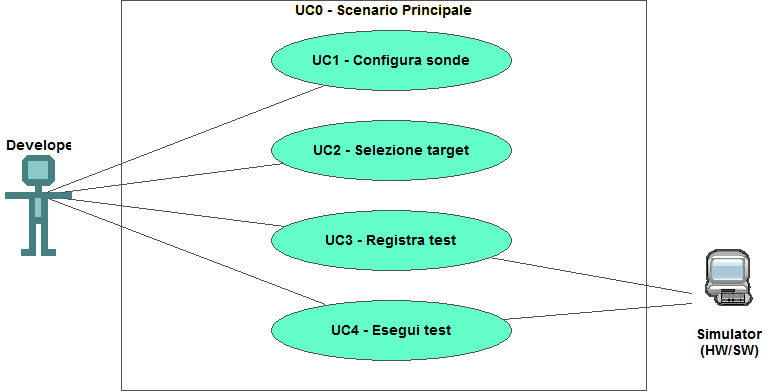
\includegraphics[width=0.9\columnwidth]{usecase/scenario-principale} 
    \caption{Use Case - UC0: Scenario principale}
\end{figure}

\begin{usecase}{0}{Scenario principale}
\usecaseactors{Sviluppatore applicativi}
\usecasepre{Lo sviluppatore è entrato nel plug-in di simulazione all'interno dell'IDE}
\usecasedesc{La finestra di simulazione mette a disposizione i comandi per configurare, registrare o eseguire un test}
\usecasepost{Il sistema è pronto per permettere una nuova interazione}
\label{uc:scenario-principale}
\end{usecase}

\section{Tracciamento dei requisiti}

Da un'attenta analisi dei requisiti e degli use case effettuata sul progetto è stata stilata la tabella che traccia i requisiti in rapporto agli use case.\\
Sono stati individuati diversi tipi di requisiti e si è quindi fatto utilizzo di un codice identificativo per distinguerli.\\
Il codice dei requisiti è così strutturato R(F/Q/V)(N/D/O) dove:
\begin{enumerate}
	\item[R =] requisito
    \item[F =] funzionale
    \item[Q =] qualitativo
    \item[V =] di vincolo
    \item[N =] obbligatorio (necessario)
    \item[D =] desiderabile
    \item[Z =] opzionale
\end{enumerate}
Nelle tabelle \ref{tab:requisiti-funzionali}, \ref{tab:requisiti-qualitativi} e \ref{tab:requisiti-vincolo} sono riassunti i requisiti e il loro tracciamento con gli use case delineati in fase di analisi.

\newpage

\begin{table}%
\caption{Tabella del tracciamento dei requisti funzionali}
\label{tab:requisiti-funzionali}
\begin{tabularx}{\textwidth}{lXl}
\hline\hline
\textbf{Requisito} & \textbf{Descrizione} & \textbf{Use Case}\\
\hline
RFN-1     & L'interfaccia permette di configurare il tipo di sonde del test & UC1 \\
\hline
\end{tabularx}
\end{table}%

\begin{table}%
\caption{Tabella del tracciamento dei requisiti qualitativi}
\label{tab:requisiti-qualitativi}
\begin{tabularx}{\textwidth}{lXl}
\hline\hline
\textbf{Requisito} & \textbf{Descrizione} & \textbf{Use Case}\\
\hline
RQD-1    & Le prestazioni del simulatore hardware deve garantire la giusta esecuzione dei test e non la generazione di falsi negativi & - \\
\hline
\end{tabularx}
\end{table}%

\begin{table}%
\caption{Tabella del tracciamento dei requisiti di vincolo}
\label{tab:requisiti-vincolo}
\begin{tabularx}{\textwidth}{lXl}
\hline\hline
\textbf{Requisito} & \textbf{Descrizione} & \textbf{Use Case}\\
\hline
RVO-1    & La libreria per l'esecuzione dei test automatici deve essere riutilizzabile & - \\
\hline
\end{tabularx}
\end{table}%

    \chapter{Progettazione e codifica}
\label{cap:progettazione-codifica}

\intro{Breve introduzione al capitolo}\\

\section{Tecnologie e strumenti}
\label{sec:tecnologie-strumenti}

Di seguito viene data una panoramica delle tecnologie e strumenti utilizzati.

\subsection*{Tecnologia 1}
Descrizione Tecnologia 1.

\subsection*{Tecnologia 2}
Descrizione Tecnologia 2

\section{Ciclo di vita del software}
\label{sec:ciclo-vita-software}

\section{Progettazione}
\label{sec:progettazione}

\subsubsection{Namespace 1} %**************************
Descrizione namespace 1.

\begin{namespacedesc}
    \classdesc{Classe 1}{Descrizione classe 1}
    \classdesc{Classe 2}{Descrizione classe 2}
\end{namespacedesc}


\section{Design Pattern utilizzati}

\section{Codifica}

    \chapter{Verifica e validazione}
\label{cap:verifica-validazione}

    \chapter{Conclusioni}
\label{cap:conclusioni}

\section{Consuntivo finale}

\section{Raggiungimento degli obiettivi}

\section{Conoscenze acquisite}

\section{Valutazione personale}


    \appendix
    \chapter{Appendice A}

\epigraph{Citazione}{Autore della citazione}


    \backmatter
    \printglossary[type=\acronymtype, title=Acronimi e abbreviazioni, toctitle=Acronimi e abbreviazioni]
    \printglossary[type=main, title=Glossario, toctitle=Glossario]

    \cleardoublepage
\chapter{Bibliografia}

\nocite{*}

% Print book bibliography
\printbibliography[heading=subbibliography,title={Riferimenti bibliografici},type=book]

% Print site bibliography
\printbibliography[heading=subbibliography,title={Siti web consultati},type=online]

\end{document}
